\chapter{Implementation}

\label{chap:impl}

% -------------------------------------------------------------------------------------------------
%                                           General TODOs
% -------------------------------------------------------------------------------------------------


\todo{Add references to documentation at appropriate places}
\todo{ add disclaimer, that most of this information was derived from reading the source code and may in some places not be accurate because the code is pretty complex and
    i have only been at it for a few months}

% TODO viruteller address raum eines xv6 processes
% Qemu implementation TLB vs Echter TLB
% -------------------------------------------------------------------------------------------------
%                                    Chapter structure overview
% -------------------------------------------------------------------------------------------------

%   Source overview
%     QEMU
%     xv6
%   Stage1 - Single Fixed address
%     Qemu - exception
%     xv6 - tlb triggerer
%   Stage2
%     Qemu - TLB CSRs
%     xv6 - Exception Handler, single address tlb fill
%       Exception vector entry -> state save, kernel stack
%   Stage3 - VM PTW with TLB miss handler
%     Qemu -> Extension to all addresses
%     xv6 -> tlb miss handler with ptw
%   Stage4 - Dynamic Segmentation allocation scheme (btw -> link to MIPS?)
%     Qemu -> No more changes needed
%     xv6 -> A lot of changes here
%   Debugging
%   Discussion on implementation
%       Concurrency
%       VM Features
% -------------------------------------------------------------------------------------------------

% High level description of the development steps and their reasoning

% -------------------------------------------------------------------------------------------------
% Section on the rationale for choosing this platform -> or just say that this was chosen and dont rationalize it

% -------------------------------------------------------------------------------------------------
% Introductory section
This chapter summarizes the implementation of the \textit{softtlb} page-table-less virtual memory system. softtlb is a term used secludedly in this paper and refers to the software handling of TLB misses via an exception handler.
The order of the sections in this chapter reflects the implementation process of the softtlb design and a mapping function implemented on top of that design. It consists of the following steps:
\begin{enumerate}
    \item \textbf{TLB miss exception and Exception Triggerer} The first step is about
          the implementation of the TLB miss exception in the QEMU RISC-V emulator. On the xv6-side,
          a user-mode program is added to trigger a TLB miss exception from the shell.
    \item \textbf{Exception Handling and TLB Writing} The second step is to implement the
          handling of the TLB miss exception by implementing a machine mode exception handler.
          The RISC-V emulation is extended by two new CSRs that facilitate writing TLB from the
          software-side of things.
    \item \textbf{Software Page Table Walk for all Addresses} This step removes the restriction
          in the QEMU emulator to only throw exceptions for a specific address. In the exception handler,
          a page table walk is implemented to now create virtual to physical mappings for all addresses.
    \item \textbf{Segmented Memory Design using software-defined TLB Filling} In this step, the xv6 virtual memory system is completely
          replaced. The new design gets rid of the page table and only uses information present in
          registers to create virtual-to-physical mappings and to fill the tlb.
\end{enumerate}
Each section elaborates on both the xv6 side and the QEMU side of the implementation.
The final section describes debugging techniques that were used or can otherwise be useful for
similar implementations.

\begin{figure*}[t!]
    \centering
    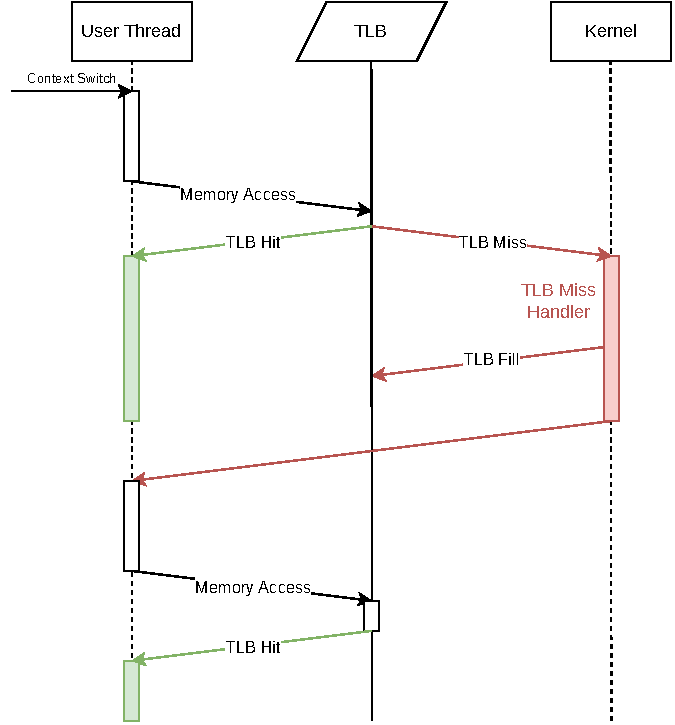
\includegraphics[scale=1]{figures/sequence.pdf}
    \caption[Sequence of actions]{Sequence of action in case of a TLB Hit and Miss}
    \label{impl:sequence}
\end{figure*}


% First step in the development process
% -------------------------------------------------------------------------------------------------
%                                          SECTION STEP 1
% -------------------------------------------------------------------------------------------------
\section{TLB miss exception and Exception Triggerer }
There are two prerequisites the hardware needs to fulfill in order to do a software-managed TLB fill:
to be a way to signal to the operating system that a TLB miss occurred and there needs to be some
sort of instruction that can be used to write TLB entries.
This step is about the former: Changing the QEMU RISC-V emulator to throw a newly defined \textit{
    TLB miss exception} whenever the TLB misses.
% Why only start with one fixed address?
Changing the whole system to start throwing a TLB miss exception on every virtual address would
make it very hard to debug both first tries at implementing a handler for the exception and the
exception throwing code in QEMU itself.
And not only would the exception be thrown as soon as virtual memory is activated in
\texttt{xv6-riscv:kernel/main.c}, the exception would be thrown
as soon as exceptions are activated and a memory access happens, because QEMU also uses the
\texttt{fill\_tlb} routine to fill the TLB with direct
virtual-to-physical mappings when no virtual memory is used. This speeds up the execution of
the dynamically translated code, as it is able to directly
lookup addresses in the TLB using a fast path \cite{DeepDiveQEMU}.
For this step of the implementation, the QEMU memory system emulation must be changed to throw a
TLB miss exception when a TLB lookup misses. To keep the system running as normal, this will
be done for only one hardcoded address, that is usually not used by xv6.
On the xv6 side, we need a user-level program, that accesses the specific address and thus prompts
the emulated hardware to throw a TLB miss exception.


% -------------------------------------------------------------------------------------------------
\subsection{Address Selection}
The choice for an address to be used for testing the TLB miss exception throwing is easy:
As shown in Figure \ref{impl:xv6layout}, the physical memory map of xv6 has an
area of ``Free memory'' that is managed by the physical memory allocator. The memory allocator
always gives out the next page starting from low to high addresses when a new page is requested
by kernel routines. The address \texttt{0x84fff000} was chosen as a testing address.
Note that the physical memory allocator in \texttt{kalloc.c} will actually reference this address(or
any address in the range from \texttt{0x80000000} to \texttt{0x88000000}), when initializing
the linked list used to keep track of the free pages \cite{cox2011xv6}.\todo{explain why this
    may be relevant or just leave it out? }
% does not need to be an accessible address now, but later we want to write and read from it

\begin{figure*}[t!]
    \centering
    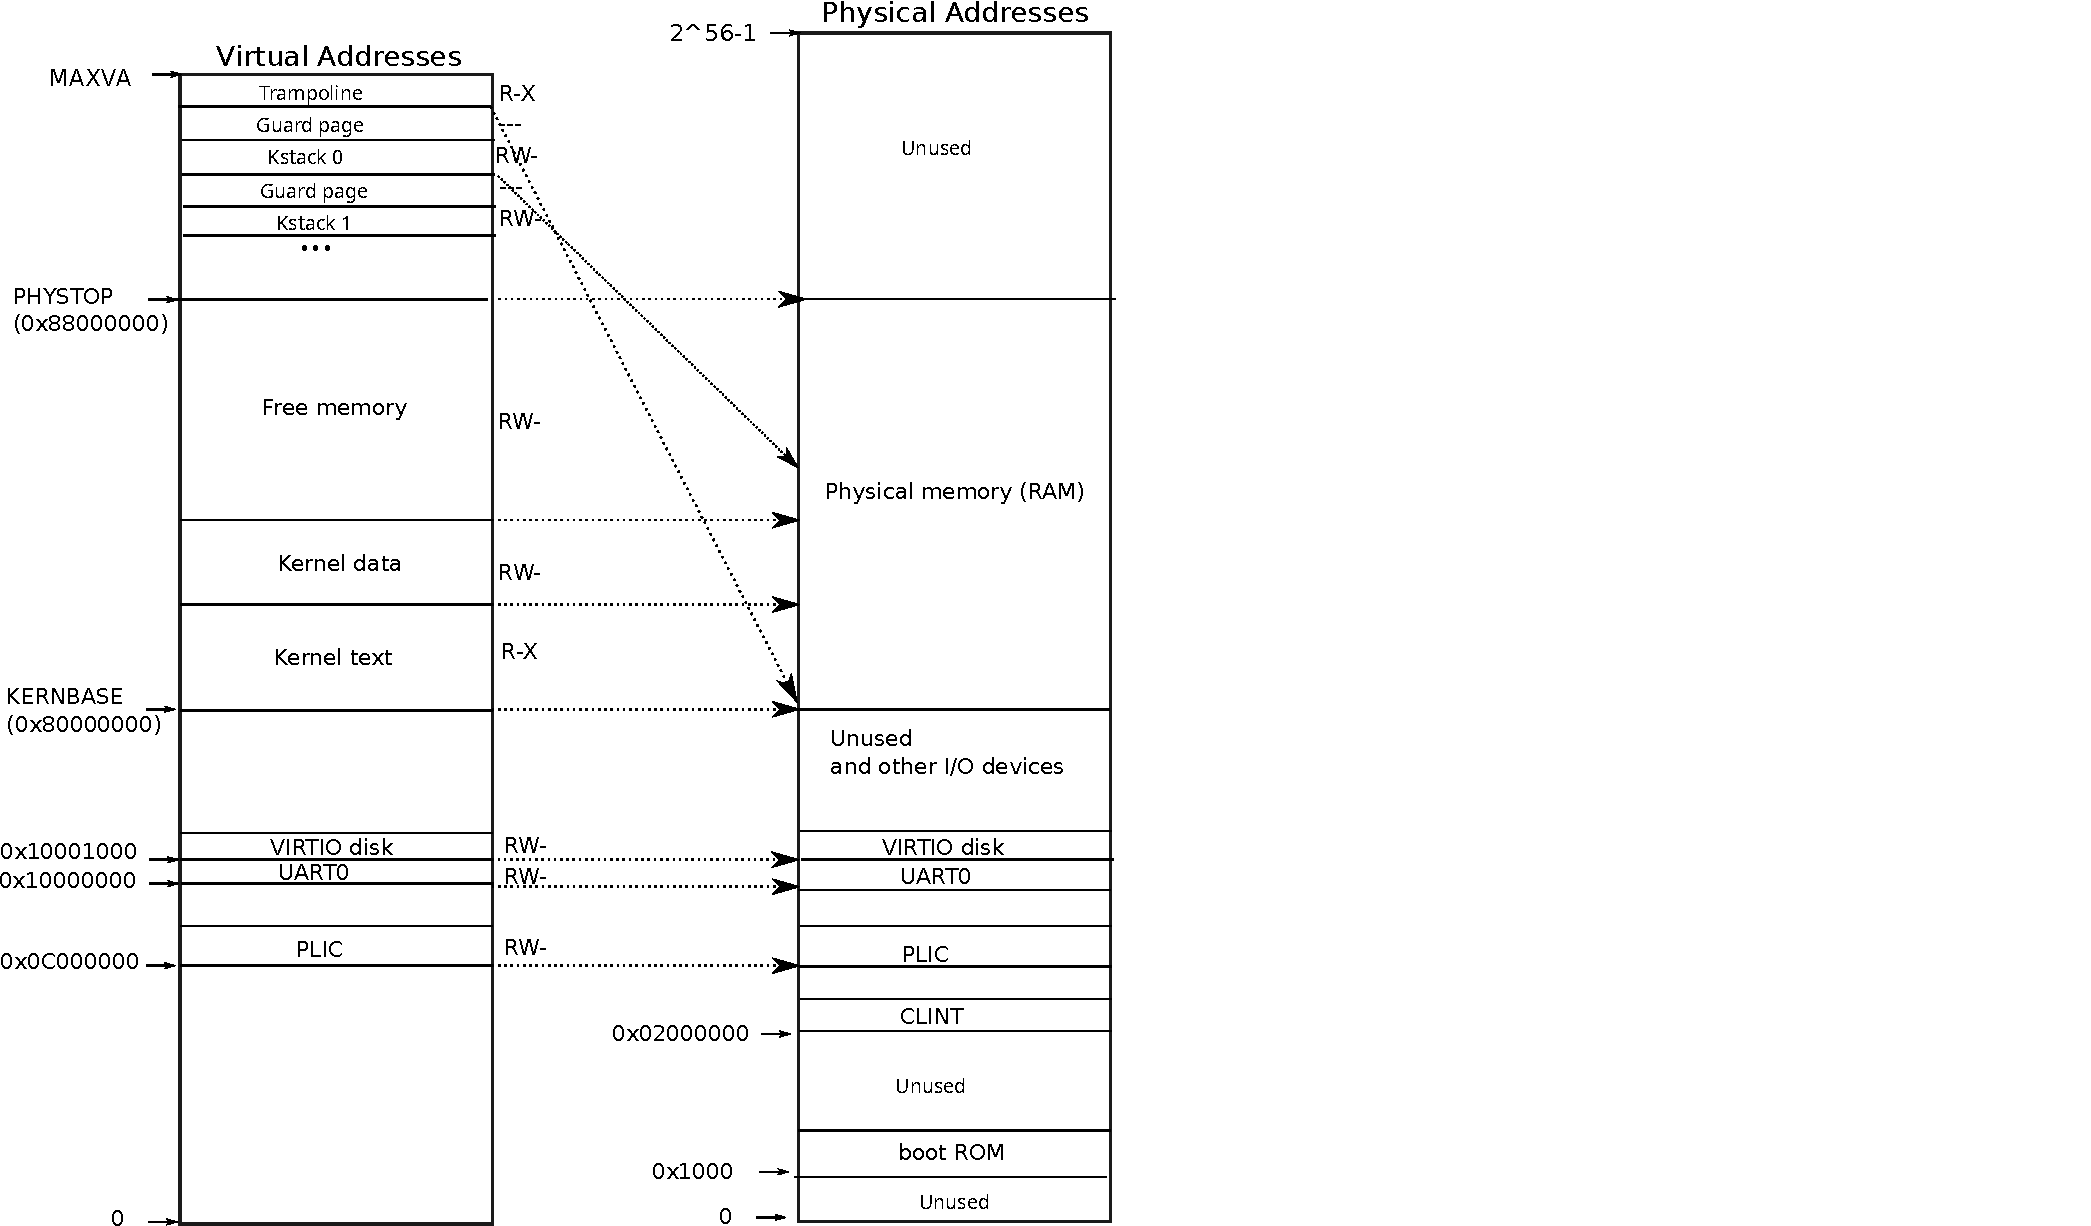
\includegraphics[scale=.5]{figures/xv6_layout.pdf}
    \caption[xv6 memory layout]{The xv6 memory layout and how the kernel virtual address space is mapped on
        the physical address space. Taken from the xv6 book \cite{cox2011xv6}.}
    \label{impl:xv6layout}
\end{figure*}


\subsection{TLB miss exception in QEMU}
%TODO Explain what the riscv_cpu_tlb_fill function does originally - in detail
% TODO discussion and reference to READER/SPECIFICATION on what exception numbers and other constants can be used and are free

% Qemu RISCV  exception adding "tutorial"
%TODO Description of the TLB Exception implementation and how to generally add exceptions to the QEMU plattform
% TODO List of code locations where changes need to be added -> should be usable as back reference for implementing more exceptions

To properly test the implementation, the \texttt{tlb\_fill} function was replaced to throw the
TLB\_MISS exception for
one specified, page-aligned address and to continue normally for every other address.
The implementation is outlined
in Listing \ref{lst:specialCaseTLBfill}.



% riscv_cpu_tlb_switch function
%TODO is this listing really interesting?
\begin{lstlisting}[language=c,float=h!,
    caption={Alternative Implementation for the RISC-V tlb\_fill function with a special case to
    start testing TLB Miss Handler implementations.
    In line 11, a conditional branch is used to only trigger the exception when neither the
    Virtual Memory (as set in the \texttt{satp} \texttt{MODE} field) is bare nor the privilege
    mode is the machine mode.
    If the virtual address is the hardcoded one, a TLB miss exception is thrown, otherwise the
    original functions is called, which will perform a page table walk to find the mapping.},
    label={lst:specialCaseTLBfill}]
bool my_riscv_cpu_tlb_fill(CPUState *cs, vaddr address, int size,
    MMUAccessType access_type, int mmu_idx,
    bool probe, uintptr_t retaddr)
{
    RISCVCPU *cpu = RISCV_CPU(cs);
    CPURISCVState *env = &cpu->env;
    int mode = mmuidx_priv(mmu_idx);
    int vm = get_field(env->satp, SATP64_MODE);
    bool ret = false;

    if(!(vm == VM_1_10_MBARE || mode == PRV_M) &&
            address == (uint64_t)0x84fff000) {
        ret = riscv_cpu_tlb_miss_exception(cs,address,size,access_type, mmu_idx, probe, retaddr);
    } else {
        ret =  riscv_cpu_tlb_fill(cs,address,size,access_type, mmu_idx, probe, retaddr);
    }
    return ret;
}
\end{lstlisting}

% -------------------------------------------------------------------------------------------------


% This section describes the necesarry steps for adding the TLB miss exception to the qemu source
%in comparison with Page fault exceptions
To draw inspiration on how to implement a TLB miss exception in QEMU, you can look at how
page fault exceptions are thrown.
Whenever a page fault exception is triggered, the TLB is checked first to see if there is a mapping
for the input virtual address \cite{QEMUSource2024}. Additionally, RISC-V cores provide the faulting
address of the page fault exception in the \texttt{mtval} register \cite{RISCVInstructionSet}.
The faulting address will also be necessary for handling the TLB miss exception.


% -------------------------------------------------------------------------------------------------

% -------------------------------------------------------------------------------------------------

% Adding new Exception to Qemu RV target
\paragraph{New Exception} Adding a new exception to the QEMU emulator requires changes at a number of places. In the following,
the relevant code locations in the QEMU source \cite{QEMUSource2024} are shown.
This may be completely different for other targets, as the exception code is mostly target specific and
this implementation only looked at the RISC-V target.
\begin{itemize}
    \item \texttt{target/riscv/cpu\_bits.h} contains all CPU-definitions specific to the RISC-V target.
          There is also an enum called \texttt{RISCVException} which contains the number-codes for all RISC-V exceptions.
          In choosing an appropriate number for a new exception, one should consult the Privileged Architecture Specification \cite{RISCVInstructionSet}.
          There are specific exception code ranges that are designated for custom use. E.g. the codes 24--32 and 48--63.
    \item \texttt{target/riscv/cpu\_helper.c\:riscv\_cpu\_do\_interrupt\(\)} is the target-specific function
          for triggering interrupts. Here it suffices to add the new exception enum item to the switch case, when
          the new exception is similar in behavior to existing exceptions.
          Here the new exception is simply supposed to jump into an exception handler in the kernel. A lot of exceptions
          like page faults share that behavior.
    \item Finally, if the exception should be delegatable to supervisor mode or user mode, the n-th bit,
          with n being the exception code, needs to be set in the \texttt{DELEGABLE\_EXCPS} definition in \texttt{target/riscv/csr.c}.
          This enables the kernel to delegate the exception to another privilege level by setting the appropriate
          bit in the \texttt{medeleg} and \texttt{sedeleg} CSRs.
\end{itemize}

The code shown in Listing \ref{lst:specialCaseTLBfill} will finally trigger the function shown in
Listing \ref{lst:exceptionThrow}. After executing this function, QEMU will trigger a TLB miss exception as soon
as it gets back to the main execution loop \cite{QEMUSource2024}.

\begin{lstlisting}[language=c,float=h!,
    caption={Setup-Code for raising a TLB Exception. The \texttt{cs-\textgreater exception\_index} variable needs
    to be set to the custom \texttt{TLB Exception} enum value. The \texttt{env-\textgreater badaddr} variable
    will end up in the \texttt{mtval} register. The address will be page-aligned first, by zeroing out the
    lowest 12 bits. This is used to encode the \texttt{mmu\_idx} into the faulting address. Why this is
    necessary is explained in Section \ref{sect:tlbwrite}},
    label={lst:exceptionThrow}]

    static void raise_tlb_exception(CPURISCVState *env, target_ulong address,
                                MMUAccessType access_type,
                                /*unnecessary?*/ bool pmp_violation,
                                bool first_stage, bool two_stage,
                                bool two_stage_indirect, uint8_t mmu_idx) {
        CPUState *cs = env_cpu(env);

        cs->exception_index = RISCV_EXCP_TLB_MISS;
        env->badaddr = ( address & ~( (1 << 12) - 1)) | mmu_idx;
        env->two_stage_lookup = two_stage;
        env->two_stage_indirect_lookup = two_stage_indirect;
    }

\end{lstlisting}

% -------------------------------------------------------------------------------------------------


\subsection{Exception Triggerer}
% TODO TLB exception trigger
To properly test the changes introduced to the QEMU emulator, there needs to be some way to
trigger a TLB exception.
By implementing this as a user-level program, the exception can be triggered using the xv6 shell.

\paragraph{New User Program} Adding a new user-level Program to xv6 only needs you to add a new \texttt{.c} file to the user subfolder
and to add the name of the generated binary ( name of \texttt{.c} file prefixed with a \texttt{\_})
to the list of user binaries in the makefile.
The new \texttt{.c} file only needs a \texttt{main} function and should also include the \texttt{user.h}
file to gain access to some preimplemented function and system call wrappers \cite{xv6source}.

The final exception triggerer may look something like this:

\begin{lstlisting}[language=c,float=h!,label{impl:excptTrigger},caption={\textbf{Exception Triggerer} Trying to
    load from a hardcoded address prompts the emulated hardware to trigger a TLB miss exception.}]
    #include "kernel/types.h"
    #include "user/user.h"

    void do_tlb_exc(void) {
        __asm__("li s2, 0x84fff000\n\t \
                lw s4, 0(s2)\n\t");
        register int *foo asm ("s4");
        printf("%x\n", foo);
        return;
    }

    int main(int argc, char *argv[]) {
        do_tlb_exc();
        //exit(0);
    }
\end{lstlisting}



The program first loads the hardcoded address into a register and then tries to load a word from this address.
If the implementation of the \texttt{TLB miss exception} was done correctly, the process will trap to the kernel
and the kernel will print out an error message, as it does for all exceptions that either have unknown exception
numbers or do not have an exception handler implemented \cite{cox2011xv6}.
If the exception was not properly implemented, the kernel would report a load page fault exception.

\todo{add xv6 shell output at this stage progression - should be an error printed by the kernel exception handler}
% -------------------------------------------------------------------------------------------------
%                                       END OF SECTION - STEP 1
% -------------------------------------------------------------------------------------------------



% Second step: Extending the tlb miss handling to be used for all addresses -> implementing a softvm ptw
% -------------------------------------------------------------------------------------------------
%                                         SECTION - STEP 2
% -------------------------------------------------------------------------------------------------
\section{Exception Handling and TLB Writing}
\label{sect:tlbwrite}

Now that the new \textit{TLB miss exception} can be triggered by a user-level program, there needs
to be an exception handler in the kernel that will create virtual-physical mappings and add them to the
TLB.
This section will first go into a general description on how to add new CSRs to the RISC-V QEMU emulation and
will then elaborate on the specific implementation for the TLB CSRs.
The section ends with the implementation of the exception handler.

% TODO Why does the mmuidx need to be encoded into the faulting address -> Explain


% -------------------------------------------------------------------------------------------------
\subsection{Adding CSRs to RISC-V/QEMU}

% Relevant Code locations
The following code locations are relevant for CSRs in the RISC-V/QEMU emulation source code \cite{QEMUSource2024}:
\begin{itemize}
    \item \texttt{disas/riscv.c} Contains a big switch case with all the CSR number to CSR name mappings.
          Name and number of new CSRs need to be added there.
    \item \texttt{target/riscv/cpu\_bits.h} contains definitions for all CSR numbers.
          While it is not strictly necessary to add another definition for new CSRs here, readability and maintainability
          of the code increases if a more descriptive definition name is used instead of a magic constant.
    \item \texttt{target/riscv/cpu\_cfg.h} contains a structure called \texttt{RISCVCPUConfig}. Every emulated RISC-V hart
          has this structure to expose all the extensions that the hart supports. \todo{hart already known?}
          The structure has a boolean flag for every extension that is currently supported by the emulator.
          New extensions should get their own flag in this struct.
          Similar entries also need to be added to the \texttt{isa\_edata\_arr} and \texttt{riscv\_cpu\_extensions} arrays in \texttt{target/riscv/cpu.c}.
    \item \texttt{target/riscv/csr.c} contains the implementation for all CSRs. The \texttt{riscv\_csr\_operations csr\_ops[]}
          array is essential for adding callback functions to CSR numbers.
          For every new CSR, a struct of the type \texttt{riscv\_csr\_operations} must be added to that array using the
          CSR number as an index. This struct is comprised of multiple function pointers, which deal with
          \begin{itemize}
              \item Checking if the hart implements the CSR
              \item Reading from the CSR
              \item Writing to the CSR
              \item Combined read/write
              \item 128 bit read/writes
          \end{itemize}
\end{itemize}
%Implementation of CSRs

As previously mentioned, the CSRs have some index ranges for new, custom CSRs. For the implementation
of TLB write CSRs, the indexes \texttt{0xBEE} and \texttt{BFF} have been selected.
Using these constants and the steps above, two new instructions\todo{are these actually instructions} can be realized.

\subsection{CSR Callback Implementation} Apart from the above-mentioned steps to add new CSRs to the emulator, the
main logic of the implementation is in the callbacks referenced in \texttt{target/riscv/csr.c}.
The implementation of these callbacks is strongly dependent on the structure of the data that is written to
the CSRs. Fundamentally, these callbacks act as a bridge between the exposed ISA and the implementation of
that instruction set in software.
As previously mentioned, two new CSRs will be needed to implement the TLB-writing. \todo{ PUT THIS IN THE THEORY PART about CSR format and number: In theory, it would
    also be possible to implement the functionality using only one CSR, by just taking the faulting address from the mtval register, but
    this paper focuses on the proof of concept of the design and not on the optimization }
The implementations
of the write-callbacks look as follows:


% Callbacks

\begin{lstlisting}[language=c,float=h!,
    label={lst:tlbh}]
    static RISCVException write_tlbh(CPURISCVState *env, int csrno, target_ulong new_val)
    {
        env->tlbh = new_val;
        return RISCV_EXCP_NONE;
    }
\end{lstlisting}
The implementation of the \texttt{tlbh} CSR write does not do anything else but saving the value
that is written to it to the environment of the CPU.
This is because the theory specifies that the TLB entry will only
be written to the TLB when the write to the \texttt{tlbl} CSR has succeeded.

\begin{lstlisting}[language=c,float=h!,
    label={lst:tlbl}]
    static RISCVException write_tlbl(CPURISCVState *env, int csrno, target_ulong pte)
    {

        target_ulong tlb_size = TARGET_PAGE_SIZE;

        CPUState *cpu = env_cpu(env);
        vaddr addr = env->tlbh;
        hwaddr paddr = ((pte & ~(PTE_RESERVED)) >> 10) << 12;

        int mmu_idx = addr & (tlb_size - 1);

        int prot = pte & (PTE_R | PTE_W | PTE_X | PTE_V );

        addr &= ~(tlb_size - 1);
        paddr &= ~(tlb_size - 1);

        tlb_set_page(cpu, addr, paddr, prot, mmu_idx, tlb_size, false);

        env->tlbh = 0;
        env->tlbl = 0;

        return RISCV_EXCP_NONE;
    }
\end{lstlisting}
\todo{all these code lines need a theoretical foundation in the fundamentals chapter (BTW, the format
    still adheres to PTEs!)}
The value written to the \texttt{tlbl} CSR adheres to the same format as the RISC-V Sv39 PTEs (As shown in section \ref{fund:sv39}).

To get the page-aligned physical address and to get rid of the access bits stored in the lower 10 bits,
the value will first be right shifted by ten and then left shifted by 12 bits.
The topmost bits are specified to be all zero, as explained in the fundamentals chapter \cite{RISCVInstructionSet}.

In line 10, the \texttt{mmu\_idx} is extracted from the lowest 11 bits of the virtual address. This is
necessary, because QEMU uses up to 16 different MMU modes with dedicated TLBs \cite{QEMUSource2024}.
Whenever QEMU performs a TLB lookup, it does so in a specific MMU mode. This MMU mode is clear when
a TLB entry is retrieved, it is however not clear when a TLB entry is written.
To still fill the correct TLB, the \texttt{mmu\_idx} is transferred to the exception handler as part
of the faulting address in \texttt{mtval} and then back to the emulator via the TLB write CSRs.

The following lines deal with extracting the protection bits from the PTE and with page-aligning
the virtual and physical addresses. Finally, a preexisting QEMU function is invoked to add
a new entry to the emulated TLB and the CSR values are cleared.
The return value \texttt{RISCV\_EXCP\_NONE} indicates that nothing out of the ordinary happened.

This is all that needs to be done to add CSRs for TLB filling to the QEMU RISC-V emulator.


\todo{discussion of implementation at the end of this chapter: shortcommings, comparison QEMU - MIPS, comparison xv6 new vm - other vm -> eval??}

% -------------------------------------------------------------------------------------------------

\subsection{TLB miss exception Handler}
% Previous state of xv6 machine mode trap handler
%   -> Only for Timer Interrupt
%   -> Small amount of saved registers
% TODO TLB fill manager
% Changes -> Vectored mode to keep timer interrupt as is, just need to move it
With capabilities to write TLB entries in place, an effective exception handler can be implemented.

\paragraph{xv6 Machine-Mode Trap Handler} The xv6 machine-mode trap handler only deals
with the timer interrupt. All other interrupts and exceptions are delegated to the supervisor
mode. This allows the trap handler to be very small and very specific to the timer interrupt \cite{cox2011xv6}.
It thus only needs to store two registers to memory to make enough room in the register file
to reset the timer and invoke the scheduler.
Adding another trap to be handled adds more complexity, as the trap number needs to be checked
and the code needs to branch to the right routines.

But it can also be completely avoided to touch the timer code at all. xv6 uses the trap vectoring
mechanism in \textit{direct} mode. In direct mode, all traps jump to the same address.
Using the \textit{vectored} mode makes all \textit{exceptions} jump to the address set
in the \texttt{mtvec BASE} field but all \textit{interrupts} set the program counter
to \texttt{BASE} plus four times the interrupt cause \cite{RISCVInstructionSet}.

So to add machine mode exception handlers with disrupting the existing code as little as possible only
requires changing the trap vectoring mode to \texttt{vectored} mode and moving the timer interrupt code
to the correct offset.

\begin{lstlisting}[language=diff]
-    w_mtvec((uint64)timervec);
+    w_mtvec((uint64)mtvec_vector_table | 0x1);
\end{lstlisting}

The changes for changing the mode are trivial. Only the one bit indicating the \texttt{vectored} mode
needs to be set.
Placing the timer vector at the correct offset from the default trap handler vector can be achieved by
filling the space between the base address and the timer vector with no-operations. The same could be
achieved with linker directives.
The interrupt number for the timer interrupt is \texttt{0x7}, this puts the timer interrupt vector
at a positive \texttt{0x1c} offset from the base address.

\begin{lstlisting}[language={[RISC-V]Assembler},float=h!,
    label={lst:defaultTrapHandler}, caption={Vectored Trap Handler Routine}]
mtvec_vector_table:
IRQ_0:
        j default_exception_handler
        nop
IRQ_1:
        j default_vector_handler
        nop
IRQ_2:
        j default_vector_handler
        nop
IRQ_3:
        j default_vector_handler
        nop
IRQ_4:
        j default_vector_handler
        nop
IRQ_5:
        j default_vector_handler
        nop
IRQ_6:
        j default_vector_handler
        nop
IRQ_7:  # timer handler
        j timervec
\end{lstlisting}

% TODO verifying the placement of addresses and symbols using the name utility

RISC-V provides 4 bytes for every interrupt request (IRQ) and the default trap handler. This is not enough
to implement proper trap handling, so these 4 bytes are typically spent jumping to a more elaborate trap
handling routine.

Now any machine-mode exception (that is not delegated to a lower-privilege mode) sets the program counter
to the address of the \texttt{mtvec\_vector\_table} label. The next jump brings the execution into
the default exception handler.
The timer interrupt will jump directly to the \texttt{IRQ\_7} label.

\paragraph{Store/Load Sandwich} The idea behind the \textit{softtlb} design is to not use as many of the five
memory references modern architectures need for a page table walk \cite{intel5LevelPaging5Level2017}. But
for a first proof of concept, it is helpful to not have to think about which registers to use and to not optimize
away all unnecessary memory references before the design even works.
That is why the first thing the default exception handler will do is to store the current state of the register
file.
This is essential so that, once returned to the context that triggered the TLB miss, execution can continue
as if nothing happened.
After storing the state and running the exception handler, the state must again be loaded into the registers.

\todo{use minipages to have text and listing side by side ? https://latex.org/forum/viewtopic.php?t=6652}
\begin{lstlisting}[language={[RISC-V]Assembler},float=h!,
    label={lst:defaultTrapHandler}, caption={Store/Load Sandwich}]
default_exception_handler:

    csrrw a0, mscratch, a0
    sd sp, 40(a0)

    ld sp, 48(a0)
    csrrw a0, mscratch, a0

    # make room to save registers.
    addi sp, sp, -256

    # save the registers to the hart stack
    sd ra, 0(sp)
    sd gp, 16(sp)
    ...
    sd t5, 232(sp)
    sd t6, 240(sp)

    addi s0, sp, 256 # Set Frame Pointer

    # ??
    # csrr t0, sscratch
    # sd t0, 8(sp)

    # TODO Pass args to fx

    # csrr a0, mtval
    # csrr a1, satp

    call machine_default_exception_handler


    # restore registers from hart stack
    ld ra, 0(sp)
    ld gp, 16(sp)
    ...
    ld t5, 232(sp)
    ld t6, 240(sp)

    addi sp, sp, 256

    csrrw a0, mscratch, a0

    sd sp, 48(a0)
    ld sp, 40(a0)

    csrrw a0, mscratch, a0
    mret

\end{lstlisting}
\todo{side by side}
Most of the load/stores have been omitted to not flood the listing.
In between the store and load blocks, the \texttt{machine\_default\_exception\_handler} C function is called. This is
where the implementation differentiates between the different exception numbers and calls exception handlers
specific to the exceptions.
In xv6, all other exceptions but the new TLB miss exception are handled in supervisor mode, so there are
no handlers for other exceptions.

\begin{lstlisting}[language={C},float=h!,
    label={lst:defaultTrapHandler}, caption={Exception Switch-Case Statement}]
    void machine_default_exception_handler() {
        switch (r_mcause()) {
            case NONE:
            case INST_ADDR_MIS:
            case INST_ACCESS_FAULT:
            case ILLEGAL_INST:
            case BREAKPOINT:
            case LOAD_ADDR_MIS:
            case LOAD_ACCESS_FAULT:
            case STORE_AMO_ADDR_MIS:
            case STORE_AMO_ACCESS_FAULT:
            case U_ECALL:
            case S_ECALL:
            case INST_PAGE_FAULT:
            case LOAD_PAGE_FAULT:
            case STORE_PAGE_FAULT:
            default:
                unhandled_exc(r_mcause(), r_mtval());
                break;
            case TLB_MISS:
                tlb_handle_miss(r_mtval(), r_satp());
                break;
        }
    }
\end{lstlisting}

Finally, the \texttt{tlb\_handle\_miss()} functions is called with the faulting address and the \texttt{satp} register
value as arguments.
The initial implementation simply calls the new \texttt{tlbh} and \texttt{tlbl} CSR instructions with and a pair of virtual and physical address and then
returns.
% Description of tlb handler and call of tlbh and tlbl
\begin{lstlisting}[language={C},float=h!,
    label={lst:defaultTrapHandler}, caption={Simple TLB miss exception handler for a single fixed address}]
void tlb_handle_miss(uint64 addr, uint64 usatp) {
  //uint64 *paddr = kalloc();
  w_tlbh(addr);
  w_tlbl((uint64)addr+(uint64)0x1000);
  return;
}
\end{lstlisting}

Note that this implementation does not yet use the format for the \texttt{tlbh} and \texttt{tlbl} CSRs specified
in the theory section \ref{chap:theory}.
Merely the faulting address and the intended mapping are written to the registers.

% HERE TODO explain the implication for implementation
\subsection{Testing}
Listing \ref{lst:defaultTrapHandler} already shows a part of the setup to test that the mapping actually worked.
When the mapping worked, it should be possible to read a value from the mapped page.
The user-level exception triggerer already tries to do just that.
With the mapping working, the output of the program looks as follows:

\todo{add console output}

The value \texttt{0xDEADBEEF} that was read from the mapped page is not a coincidence:
For testing purposes, the page \texttt{0x85000000} was filled with \texttt{0xDEADBEEF} bit patterns.

The address for the physical ''testing'' page was deliberately chosen to be \texttt{0x85000000} and not
\texttt{0x84fff000} (like all the hardcoded testing addresses) to make sure that there is no accidental physical
mapping happening.


\todo{add xv6 shell output at this stage progression - no more exception printing, xv6 should read deadbeef now}

% -------------------------------------------------------------------------------------------------
%                                       END OF SECTION - STEP 2
% -------------------------------------------------------------------------------------------------



% -------------------------------------------------------------------------------------------------
%                                       STEP 3 - New VM
% -------------------------------------------------------------------------------------------------
\section{Software Page Table Walk for all Addresses}
After implementation step 2, we now have a modified QEMU RISC-V emulator, which will throw the new
TLB miss exception when the TLB misses.
We have also extended the xv6 operating system to catch said exception and to create a virtual-physical
mapping for the faulting address.
The mapping is created by writing new TLB entries using newly implemented TLB CSRs.

Currently, all of this only works for one specific ''testing'' address. This step now elaborates on
how the scheme is extended to be used for all addresses.
To not change too much at once, the page table walk that would typically be done in hardware is
implemented as part of the TLB miss exception handler.

\subsection{TLB miss exception for all Addresses}
The changes introduced to QEMU are simple: Essentially, only the condition checking if the given address is
the ''testing'' address needs to be changed.
The final implementation looks as follows:

\begin{lstlisting}[language=c,float=h!,
    caption={},
    label={lst:updatedTLBFill}]
    bool my_riscv_cpu_tlb_fill(CPUState *cs, vaddr address, int size,
                        MMUAccessType access_type, int mmu_idx,
                        bool probe, uintptr_t retaddr)
    {
        RISCVCPU *cpu = RISCV_CPU(cs);
        CPURISCVState *env = &cpu->env;
        int mode = mmuidx_priv(mmu_idx);
        int vm = get_field(env->satp, SATP64_MODE);

        //No address translation in m-mode
        if(vm == VM_1_10_MBARE || mode == PRV_M) {
            int tlb_size = 4096; //TODO Get from PMP?
            hwaddr pa = address;
            int prot = PAGE_READ | PAGE_WRITE | PAGE_EXEC;
            tlb_set_page(cs, address & ~(tlb_size - 1), pa & ~(tlb_size - 1),
                        prot, mmu_idx, tlb_size, true);
            return true;
        }
        riscv_cpu_tlb_miss_exception(cs,address,size,access_type, mmu_idx, probe, retaddr);
        return true;
    }
\end{lstlisting}

Note that in comparison to the previous implementation (as shown in figure \ref{lst:specialCaseTLBfill}), the
call to the original \texttt{riscv\_cpu\_tlb\_fill} function is not called anymore.
Either a TLB miss exception is raised, or the TLB is filled with an identity mapping if either the current
privilege mode is the machine mode or the virtual memory system is configured to use identity mappings only
\cite{RISCVInstructionSet}.

% -------------------------------------------------------------------------------------------------

\subsection{Software Page Table Walk}


\begin{figure*}[ht!]
    \centering
    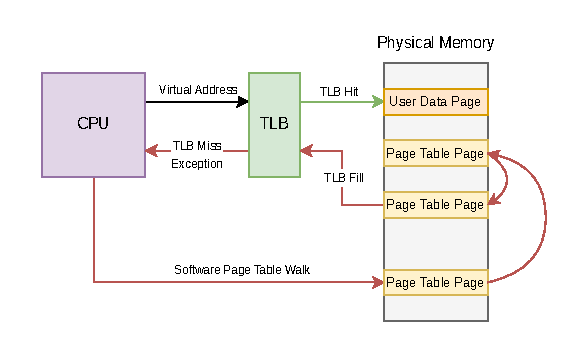
\includegraphics[scale=1.5]{figures/theory_sw_ptw.pdf}
    \caption[Software Page Table Walker]{Instead of transfering control over to the MMU to fill in the missing mapping,
        the TLB miss exception invokes a software page table walker}
    \label{fig:theory:sw_ptw}
\end{figure*}

Now that the TLB miss exception is thrown for every faulting address, it also needs to be handled
for every address.
Even though the goal is to explore alternatives to virtual memory using page tables, we will
use a software implementation of the hardware page table walk. This is to verify that the
general setup including exception invocation, exception handling and TLB writing works as
expected.
Listing \ref{lst:softptw} shows the implementation.

\todo{The listing seems to be way broader than it needs to be}
\begin{lstlisting}[language=c,float=t,
    caption={\textbf{TLB miss exception Handler with Page Table Walk}
    The \texttt{walk\_pt()} function walks the Sv39 page table with the base address
    encoded in the \texttt{satp} register. If a PTE with the valid bit set is found, the function
    returns the address encoded in the PTE.
    Otherwise, the function returns \texttt{0}.},
    label={lst:softptw}]
#define SATP2PA(satp) ((satp << 12) & ~(0xffull << 44))

pte_t *
walk_pt(uint64 satp, uint64 va)
{
  uint64 *pt = (uint64*)SATP2PA(satp);
  if(va >= MAXVA)
    panic("walk");
  for(int level = 2; level > 0; level--) {
    pte_t *pte = &pt[PX(level, va)];
    if(*pte & PTE_V) {
      pt = (uint64*)PTE2PA(*pte);
    } else {
      return 0;
    }
  }
  return &pt[PX(0, va)];
}

void tlb_handle_miss(uint64 addr, uint64 satp) {
    w_tp(r_mhartid());
    pte_t *pte = walk_pt(satp, addr);
    w_tlbh(addr);
    uint16 prot =  PTE_R | PTE_W | PTE_U | PTE_V;
    w_tlbl(*pte | prot);
    return;
}
\end{lstlisting}

\todo{To make it easier to understand -> Architectural overview of the memory path after each implementation step?}

If the \texttt{walk\_pt()} function returns 0, the virtual address lead to no valid PTE. This is a
page fault and would raise a page fault fitting the faulting instructions type of access \cite{tanenbaumOS}.
As xv6 does not handle page faults other than by killing the program \cite{cox2011xv6} this
paper will not go into more detail of raising and triggering page faults for the \texttt{softtlb}
design.


% -------------------------------------------------------------------------------------------------
%                                               STEP 4
% -------------------------------------------------------------------------------------------------

\section{Segmented Memory Design using software-defined TLB Filling}

After step 3, xv6's virtual memory system runs completely without using the (emulated) page table
walking state machine:
Instead of invoking the page table walker, a TLB miss triggers an exception. This exception is handled by the
operating system kernel and a TLB entry for the faulting address is generated.
Yet at this point, we have not really won anything. We only moved the page table walking to the software side,
which would certainly be slower at traversing the page table than a real MMU \cite{jacob1998look}. And that is
even if we ignore the expensive context switch that needs to be performed when the exception handler is invoked.

While we did not gain any performance, there is now the opportunity to modify the virtual memory system
completely in software. We do not need to adhere to the rigid structures \cite{tanenbaumOS} of the memory management hardware anymore.
We gained a great deal of flexibility.

The rest of this section explores a first idea of how a table-based virtual memory system can be
replaced by essentially a simple function that does not require expensive memory accesses.

The initial idea, as presented in the theory chapter, is a segmented memory design. It splits the total
available memory into parts of equal size, also called segments.
Each new process acquires one of those segments, if there are any left. If none are left, process creation fails.

\todo{basic assumption to make this work: xv6 process memory model -> should be mentioned here and explained in detail in theory}
% TODO Concept of AS used here -> distinct from hard ware mechanism, but could be used for it
\subsection{Address Spaces}
As with segmentation, the available physical memory is split into evenly sized portions\todo{is it? Cite!}
from now called address spaces. When a new process is started it tries to acquire an address space by
checking whether there is a free one and then claiming that free address space.
The number of address spaces will thus limit the number of concurrently running programs.

To keep track of which process acquired which address space, the kernel keeps an integer array of process IDs.
This array has a size equal to the number of address spaces (NAS).
For a newly created process to acquire an address space, the kernel will (synchronized by a spinlock \cite{cox2011xv6})
iterate through the array to find an array slot with the value 0. It then writes the process ID into that array.
The process creation fails if there are no more array slots set to 0.
The address space ID (ASID) acquired by the process is also written to the processes control block (PCB).

NAS is set via a preprocessor definition and thus set at compilation time. More elaborate implementations
could also allow dynamic resizing of address spaces to provide space for more processes.

Using the ASID, the address range for a process can be calculated very easily. The macros in listing \ref{lst:macros}
are used in different parts of the code to calculate different addresses related to an Address Space.

\begin{lstlisting}[language=c,float=h!,
    label={lst:macros}]
    #define MAX_AS_MEM ((((PHYSTOP - (PGROUNDUP((uint64)end))) / (NAS + 1)) >> 12 )<< 12)
    #define AS_START(asid) (PGROUNDUP((uint64)end) + ((asid) * MAX_AS_MEM))
    #define AS_N(index, asid) (PROC_START(asid) + (index * (0x1000)))
    #define AS_END(asid) ((PGROUNDUP((uint64)end) + ((asid + 1) * MAX_AS_MEM))-0x1000)
\end{lstlisting}

\subsection{Mapping function for Segmented Memory}
The ASID of a process is the foundation for calculating the virtual to physical mapping in the exception handler.
The only other information required is the faulting address.
\todo{theory needs to explain that the asid is transfered via SATP reg}

The ASID can be used to calculate the actual physical address at which the Address Space starts.
The faulting address, which would, according to the xv6 process memory model, be an address in the low
end of the virtual memory space, will provide the offset into the Address Space.

Listing \ref{lst:handler} shows the implementation for the TLB miss exception handler.

\begin{lstlisting}[language=c,float=h!,
    label={lst:handler}]
#include "defs.h"
#include "param.h"
#include "types.h"
#include "riscv.h"
#include "memlayout.h"

#define SATP2ASID(satp) ((satp << 4) >> 48)

extern char trampoline[];
paddr get_mapping(vaddr addr, uint16 asid) {

  //special case for trampoline, which is in every address space at the same address
  // (except for the physical one!)
  if(PGROUNDDOWN(addr) == TRAMPOLINE) {
    return (uint64)trampoline;
  }
  if(asid == 0) {
    //Kernel -> direkt mapping
    //TODO special mappings
    return addr;
  } else {
    //mappings for processes
    //TODO trapframe and trampoline mappings
    if(PGROUNDDOWN(addr) == TRAPFRAME) {
      return TRAPFRAME_FROM_ASID(asid);
    }

    //Base case
    uint64 vpage = PGROUNDDOWN(addr);
    if(vpage >= MAX_AS_MEM - (0x1000 * 4)) {
      //Error, address out of range
      panic("tlb_manager: address to high!");
    }
    return AS_START(asid) + vpage;
  }
  return 0;
}

void tlb_handle_miss(vaddr addr, uint64 satp) {
  w_tp(r_mhartid()); //fix problems with locks based on cpuid()

  //TODO Locks!
  //TODO buffering printer, only prints completed lines
  //uint16 mmuid = addr & 0xfff;
  vaddr addr_no_mmuid = addr & ~0xfff;
  //printf("tlb_manager: addr=%p satp=%p mmuid=%d\n", addr_no_mmuid, satp, mmuid);
  paddr pa = get_mapping(addr_no_mmuid, SATP2ASID(satp));

  w_tlbh(addr);
  //TODO all access rights for now
  uint16 prot =  PTE_R | PTE_W | PTE_X | PTE_V | ((SATP2ASID(satp) != 0) ? PTE_U : 0);
  w_tlbl(PA2PTE(pa) | prot);
  return;
}
\end{lstlisting}

\todo{check tex comments here}
% TODO it is not enough to simply change the tlb miss manager, because other
%   parts of te OS still use the VM system for stuff
%       What are these parts that interact with the os?
%       How can be made it fit this scheme?

\subsection{Special Mappings}
xv6 needs a trampoline page mapped into the address space of the process for system calls to work properly (see chapter \ref{chap:theory}).
In both the kernel and in the user processes, it is mapped to the highest possible, virtual page.
If an address on this page is encountered, the handler will map it to the physical address of the trampoline page.
The handler takes the same approach for the \texttt{TRAPFRAME} page set just below the trampoline.

\subsection{Further Changes to the OS}
Other than the exception handler, other parts of the OS need to be changed to fit the new memory management scheme.

\paragraph{Physical Memory Allocator} % Rewrite below version in new context
Demand paging of the virtual memory system was the main customer of the physical memory allocator.
But some modules like the virtio disk and pipes also rely on being able to access physical pages. Thus, it is not
possible to get rid of the physical allocator completely.
Here, its managed memory is merely reduced by assigning it the memory area of the Address Space with index 0.

\paragraph{\texttt{copyin() copyout()}} The copyin() and copyout() functions are used to copy data between
user space and kernel. They traverse the page table tree to acquire the physical location for the data
to be either copied in or copied out.
Both of those function rely on the \texttt{walkaddr()} function to do the walking for them.
The implementation can be changed to call the \texttt{tlb\_manager.c:walk\_addr()} function instead.

\paragraph{Process Loading} % No page table creation, asid allocation, also no destruction, % Parsing elf directly into AS
\todo{write}
\paragraph{sbrk()}The \texttt{sbrk()} system call is used by the program to increase the size
of the programs data segment. Typically, this call would demand a new page from the physical memory allocator
and then add a new PTE to the page table.
This system call normally returns the previous program break if it was successful (so basically a pointer to
the new program area) and \texttt{-1} if it was not successful.
Instead, this design checks if the program size would increase to be bigger than the maximum program size and
then returns \texttt{-1} if it is. Else it will return the previous program break, which is also a pointer to the new memory area \cite{rochkind2004advanced}.


% -------------------------------------------------------------------------------------------------
%                                    END OF SECTION - Step 4
% -------------------------------------------------------------------------------------------------



% TODO Should this be an appendix?
% -------------------------------------------------------------------------------------------------
%                                         SECTION - Debugging
% -------------------------------------------------------------------------------------------------
\section{Debugging}
When making simultaneous changes to both the Qemu emulator and xv6, it can be difficult to determine where bugs originate from. This section first describes how to debug Qemu and xv6 individually and then outlines a combined debugging process. This can be useful, for example, when trying to trace the code path between software and emulated hardware. This is not a guide on using GDB but rather a collection of specific tricks that were useful for debugging the code in this work. Perhaps they will also be helpful in other scenarios.

\subsection{xv6}
The Makefile in the xv6-riscv source repository has a rule \texttt{qemu-gdb} to start xv6 in Qemu with a GDB server. In another terminal, you can then start GDB with the binary you want to debug and connect to the gdbstub using \texttt{target remote:<port>}. A comment in the Makefile suggests that this rule is intended for user-mode debugging, but nothing prevents you from also debugging the kernel, which is particularly useful when making changes to the memory system.

\paragraph{Debugging user mode} When debugging a user-mode program, you often want to start at the \texttt{main} function. If you set a breakpoint at this function, a breakpoint is set at a rather low virtual address. If you set the breakpoint before even starting the kernel, you might stop immediately after starting. This happens because you're currently in the Qemu boot ROM, which is mapped by Qemu into the emulated memory layout in the range \texttt{0x0 - 0x1000}. The debugger does not differentiate between virtual and physical addresses and simply looks at what the program counter (PC) contains. \todo{The satp PPN field could be used for more information (process VM configuration).}

\paragraph{Debugging the kernel} After replacing the virtual memory system, an interesting effect was observed when debugging the kernel: As soon as the \texttt{satp} register is set in the \texttt{kvminithart()} function, GDB can no longer display the code at the current address (or any following ones). This is due to the value of the \texttt{satp} register. After the VM system was redesigned, it no longer contains the \texttt{PPN}. Only the \texttt{MODE} and \texttt{ASID} fields are relevant for the new system. There is no longer a page table that the PPN could point to. This behavior suggests that the gdbstub implemented by Qemu performs a hardware-emulated page walk to obtain the physical addresses and, consequently, the code. This, of course, does not work without a page table. One way to debug the kernel properly in GDB again would be to rebuild the kernel page table as before. However, since all the kernel mappings are direct mappings, it is sufficient to place a PTE for the address \texttt{0x80000000}, where the kernel code begins, behind the PPN in \texttt{satp}.

A whole page was allocated in the code as follows:
\begin{lstlisting}[language=c,float=h!, label={lst:fake_pt}]
    uint64 *pt = (uint64*)kalloc();
    for(uint64 i = 0 ; i < 512; i++) {
      pt[i] = 0xffffffffffffffff;
    }
    pt[2] = ((0x80000000 >> 2)| PTE_V | PTE_X | PTE_W | PTE_R);
\end{lstlisting}
However, it would also be sufficient to allocate only the space for a single PTE. The PPN must be set so that at least the entry at index 2 is present. Interpreting the address \texttt{0x80000000} as a virtual address yields a value of 2 for the \texttt{VPN[2]} field. By marking this top-level page table entry as valid, the memory at this address is treated as a 1 GB superpage. This is enough to cover the kernel code, and the code can once again be viewed as usual during debugging.

\paragraph{Verifying Addresses in Binaries} Implementing the vectored trap vectoring mode
required moving the interrupt handler code for the timer interrupt to a specific offset
from the address specified in the \texttt{mtvec} \texttt{BASE} field.
To verify the correct placement of the label, the unix \texttt{nm} tool is very useful:
It lists the symbols of an object file and their addresses.
Looking back at the code in listing \ref{lst:defaultTrapHandler}, the label \texttt{IRQ\_7}
is supposed to come exactly \texttt{0x1c} bytes after the \texttt{mtvec\_vector\_table} label.

The following call confirms the correct placement of the symbols:

\begin{lstlisting}[language={sh}]
    $ nm kernel/kernel | grep 'mtvec_vector_table\|IRQ_7'
    00000000800092cc t IRQ_7
    00000000800092b0 T mtvec_vector_table
\end{lstlisting}

\todo{forktest for testing number of address spaces}
% -------------------------------------------------------------------------------------------------

\subsection{QEMU Monitor}
With the Qemu monitor, all kinds of information about the running emulation can be displayed. Particularly interesting for this work would be the monitor for the mappings currently contained in the emulated TLB. However, for RISC-V, this was not available.

\todo{Beschreibung der TLB strukturen früher im kapitel}

% -------------------------------------------------------------------------------------------------

\subsection{QEMU Record/Replay}
QEMUs Record/Replay feature allows a deterministic replay of a machine's execution by recording
all non-deterministic events that happened. This can be especially helpful to investigate bugs
that occur as a result of an interrupt or require special preconditions or timings to occur.
With the Record/Replay feature, it is easy to recreate the situation in which a bug or unexpected
behavior occured.
For this project, especially the mouse and keybord input and the hardware clock are interesting
non-deterministic events that influence the execution of the system \cite{RecordReplayQEMU}.

\subsection{Double GDB Setup}
\todo{wite}

% -------------------------------------------------------------------------------------------------
%                                    END OF SECTION - Debugging
% -------------------------------------------------------------------------------------------------


% -------------------------------------------------------------------------------------------------
% -------------------------------------------------------------------------------------------------
%                                           END OF CHAPTER
% -------------------------------------------------------------------------------------------------
% -------------------------------------------------------------------------------------------------



